\iffalse
\let\negmedspace\undefined
\let\negthickspace\undefined
\documentclass[journal,12pt,onecolumn]{IEEEtran}
\usepackage{cite}
\usepackage{amsmath,amssymb,amsfonts,amsthm}
\usepackage{algorithmic}
\usepackage{graphicx}
\usepackage{textcomp}
\usepackage{xcolor}
\usepackage{txfonts}
\usepackage{listings}
\usepackage{enumitem}
\usepackage{mathtools}
\usepackage{gensymb}
\usepackage{comment}
\usepackage[breaklinks=true]{hyperref}
\usepackage{tkz-euclide} 
\usepackage{listings}
\usepackage{gvv}                                        
\def\inputGnumericTable{}                                 
\usepackage[latin1]{inputenc}                                
\usepackage{color}                                            
\usepackage{array}                                            
\usepackage{longtable}                                       
\usepackage{calc}                                             
\usepackage{multirow}                                         
\usepackage{hhline}                                           
\usepackage{ifthen}                                           
\usepackage{lscape}
\usepackage{siunitx}
\usepackage{flushend}
\usepackage[siunitx]{circuitikz}
\usepackage{caption}

\newtheorem{theorem}{Theorem}[section]
\newtheorem{problem}{Problem}
\newtheorem{proposition}{Proposition}[section]
\newtheorem{lemma}{Lemma}[section]
\newtheorem{corollary}[theorem]{Corollary}
\newtheorem{example}{Example}[section]
\newtheorem{definition}[problem]{Definition}
\newcommand{\BEQA}{\begin{eqnarray}}
	\newcommand{\EEQA}{\end{eqnarray}}
\newcommand{\define}{\stackrel{\triangle}{=}}
\theoremstyle{remark}
\newtheorem{rem}{Remark}
\begin{document}
	
	\bibliographystyle{IEEEtran}
	\vspace{3cm}
	
	\title{GATE EE Q.17}
	\author{EE23BTECH11203 - Adarsh A$^{*}$% <-this % stops a space
	}
	\maketitle
	%\newpage
	\bigskip
	
	\renewcommand{\thefigure}{\theenumi}
	\renewcommand{\thetable}{\theenumi}
	
	
	\vspace{0.2cm}
	\linespread{1.1}
	
	
	\textbf{ Question : }
	 A continuous-time system that is initially at rest is described by,
	\begin{center}
		$\dfrac{dy(t)}{dt} + 3y(t) = 2x(t)$
	\end{center}
	where $x(t)$ is the input voltage and $y(t)$ is the output voltage.\\ 
	The impulse response of the system is?
	
	\vspace{0.2cm}
	
	(A) 3$e^{-2t}$
	
	\vspace{0.3cm}
	
	(B) $\dfrac{1}{3}e^{-2t} u(t)$
	
	\vspace{0.3cm}
	
	(C) 2$e^{-3t} u(t)$
	
	\vspace{0.2cm}
	
	(D) 2$e^{-3t}$ \hfill(GATE 2023 EE)
	
	\vspace{0.2cm}
	
	\solution
	\fi
	\begin{table}[htbp]
	\centering
	\noindent
	\fontsize{10}{15}\selectfont {
		\resizebox{0.45\textwidth}{!}{%
			\begin{tabular}{|c|c|c|}
				\hline
				\textbf{Parameter} & \textbf{Value} & \textbf{Description} \\
				\hline
				$x\brak t$ & - & Input voltage \\
				\hline
				$y\brak t$ & - & Output voltage \\
				\hline
				$h\brak t$ & $\frac{y\brak t}{x\brak t}$ & Impulse response \\
				\hline
				$X\brak s$ & - & Input voltage in s-domain \\
				\hline
				$Y\brak s$ & - & Output voltage in s-domain \\
				\hline
				$H\brak s$ & $\frac{Y\brak s}{X\brak s}$ & Impulse response in s-domain \\
				\hline
			\end{tabular}
	} }
	\caption*{Input Table}
	
\end{table}
	
	%\vspace{-0.3cm}
	
	Given equation is,
	\begin{align}
		\dfrac{dy(t)}{dt} + 3y(t) &= 2x(t)
	\end{align}
	
	Applying Laplace transform,
	\begin{align}
		x\brak{t} &
		\xleftarrow[]{\hspace{0.4cm}{\mathcal{L}}\hspace{0.1cm}}\xrightarrow[]{}
		X\brak{s}\\
		y\brak{t} &
		\xleftarrow[]{\hspace{0.4cm}{\mathcal{L}}\hspace{0.1cm}}\xrightarrow[]{}
		Y\brak{s}
	\end{align}
	
	
	%\vspace{0.5cm}
	
	From the differentiation property,
	
	\begin{align}
		\dfrac{dy\brak t}{dt} &
		\xleftarrow[]{\hspace{0.4cm}{\mathcal{L}}\hspace{0.1cm}}\xrightarrow[]{}
		s Y\brak{s}
	\end{align}
	%\vspace{0.4cm}
	The equation becomes,
	\begin{align}
		s Y\brak s + 3 Y\brak s &= 2 X\brak s\\
		Y\brak s \brak {s + 3} &= 2 X\brak s\\[5pt]
		H\brak s &= \dfrac{Y\brak s}{X\brak s}\\[5pt]
		H\brak s &= \dfrac{2}{s + 3}
	\end{align}
	\begin{align}
		\dfrac{1}{s + a} &
		\xleftarrow[]{\hspace{0.4cm}{\mathcal{L}}\hspace{0.1cm}}\xrightarrow[]{}
		e^{-at} u\brak t
	\end{align}
	
	Using these results,
	\begin{align}
		h\brak t &= 2 e^{-3t} u\brak t 
	\end{align}
	
	%\vspace{0.2cm}
	
	%\underline{Plot of $h\brak t$ $vs$ $t$} :
	
	\begin{figure}[htbp]
		\centering
		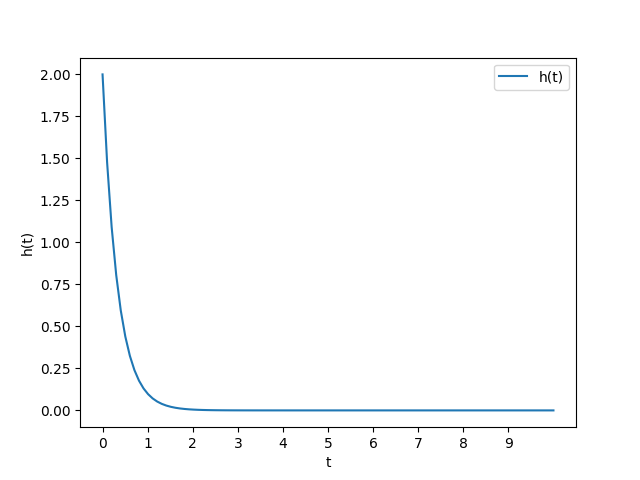
\includegraphics[width=0.6\textwidth]{2023/EE/17/figs/figure1.png}
		\caption{(a) Plot of $h\brak t$ $vs$ $t$}
	\end{figure}
	
%\end{document}
